\documentclass[11pt]{article}
\usepackage[margin=1in]{geometry}
\usepackage{amsmath,amssymb,amsthm}
\usepackage{tikz}
\usetikzlibrary{arrows.meta,positioning,calc,shapes.geometric,fit}
\usepackage{hyperref}
\usepackage{booktabs}
\usepackage{xcolor}

\newtheorem{definition}{Definition}
\newtheorem{proposition}{Proposition}

\title{Implementation Plan, PMP, WFA Classification, and the RDMA-Compute Interface\\[4pt]
\large Adaptive RDMA Optimization for Distributed LLM Training and Inference on Consumer Hardware}
\author{Nathan Gopee\\MS Computer Science Candidate, SUNY New Paltz\\\texttt{gopeen1@newpaltz.edu}\\[4pt]Advisors: Dr.\ Wafi Danesh \& Dr.\ Ashley Suchy}
\date{March 31, 2026}

\begin{document}
\maketitle
\tableofcontents
\newpage

\section{Problem Context}

Updates 1--3 cover the hardware testbed, problem statement, tensor cache architecture, and transport abstractions. This update adds the implementation, PMP control theory, and benchmark results.

\subsection{The KV Cache Problem}

Without a KV cache, every decode step recomputes attention over the entire sequence (quadratic cost). The KV cache makes decode linear by caching previous tokens' key/value projections.

The cost is memory. For $L$ layers, $K$ KV heads, head dimension $H$, sequence length $S$, FP16:
\[
\text{KV cache per request} = 2 \times L \times K \times H \times S \times 2 \text{ bytes}
\]
For a 70B model ($L{=}80$, $K{=}8$ GQA, $H{=}128$, $S{=}4096$): 1.3~GB per request. With 16 concurrent users, 21~GB of KV cache alone on a 24~GB RTX 3090.

In disaggregated serving (prefill on Cerberus, decode on Chimera), this entire cache must cross the 10GbE link ($\sim$1.2 GB/s). On InfiniBand this takes milliseconds. On our testbed it takes seconds. Compression (LoRC, KVTC, TurboQuant) reduces the payload; the dual QP pool reduces the queuing delay. Each targets a different factor in total transfer time (Equation~\ref{eq:ttft}).

\subsection{What This Update Adds}

UCX, NIXL, and NCCL treat all traffic equally or route by message size alone. They cannot distinguish a latency-critical decode activation from a background KV prefetch of the same size.

This update adds \textbf{tensor-aware RDMA traffic management}. The WFA classifier labels each transfer by its role in the inference pipeline, and the PMP bang-bang controller allocates bandwidth between priority classes. Traffic routes to separate RDMA queue pairs: a hot pool for latency-sensitive transfers, a cold pool for throughput. We validate with real RDMA writes on SoftRoCE.

\section{Theoretical Foundation}

\subsection{The Scaling Book's Decode Latency Model}

Austin et al.~\cite{scaling_book} derive the decode step time as a function of KV cache size:
\begin{equation}
T_{\text{step}} = \underbrace{\frac{B \times \text{KV}_{\text{size}}}{W_{\text{HBM}}}}_{\text{attention (always BW-bound)}} + \underbrace{\max\!\left(\frac{2B \times P}{C_{\text{FLOPs}}},\ \frac{P_{\text{bytes}}}{W_{\text{HBM}}}\right)}_{\text{MLP (can be compute-bound)}}
\label{eq:step}
\end{equation}
Decode attention has arithmetic intensity $\approx$1 (one dot product per KV byte loaded), so it is always memory-bandwidth-bound. The MLP term transitions at $B_{\text{crit}} = C_{\text{FLOPs}} / W_{\text{HBM}}$~\cite{scaling_book}. For disaggregated serving, TTFT adds the network transfer:
\begin{equation}
T_{\text{TTFT}} = T_{\text{prefill}} + T_{\text{KV transfer}} + T_{\text{first decode step}}
\label{eq:ttft}
\end{equation}
The thesis targets $T_{\text{KV transfer}}$. On a bandwidth-bound 10GbE link, $T_{\text{KV transfer}} = \text{KV}_{\text{bytes}} / W_{\text{net}}$. Every optimization maps to a specific term:

\begin{table}[ht]
\centering\small
\begin{tabular}{lll}
\toprule
\textbf{Tool} & \textbf{Term reduced} & \textbf{Mechanism} \\
\midrule
Triton / Pallas / K-Search & $T_{\text{prefill}}$, $T_{\text{decode step}}$ & Better kernel $\to$ closer to compute roofline \\
GQA / MQA~\cite{shazeer2019mqA,ainslie2023gqa} & $\text{KV}_{\text{size}}$ in Eq.~\ref{eq:step},~\ref{eq:ttft} & Fewer KV heads $\to$ smaller cache per layer \\
LoRC~\cite{zhang2024lorc} & $\text{KV}_{\text{size}}$ & SVD on $W_K, W_V$ $\to$ lower-dim KV vectors \\
KVTC~\cite{kvtc2024} / TurboQuant~\cite{turboquant2026} & $\text{KV}_{\text{bytes}}$ & Quantize + entropy-code the KV tensors \\
Dual QP pool & $T_{\text{KV transfer}}$ & Prevent head-of-line blocking on 10GbE \\
PMP controller & $T_{\text{KV transfer}}$ & Optimal bandwidth allocation across QPs \\
PTX warp specialization~\cite{dhmnr_ptx} & $T_{\text{prefill}}$ overlap & $\max(T_{\text{math}}, T_{\text{comms}})$ not sum \\
Paged Attention~\cite{vllm_paged} & $\text{KV}_{\text{bytes}}$ & Transfer only populated pages, not padded \\
Layer-by-layer xfer~\cite{chen2025transferengine} & $T_{\text{KV transfer}}$ overlap & Pipeline prefill layers with RDMA writes \\
\bottomrule
\end{tabular}
\caption{Each optimization maps to a specific term in the TTFT equation.}
\end{table}

\subsection{PMP: Bang-Bang QP Allocation}

Zhang et al.~\cite{zhang2024optcontrol} reinterpret LoRA matrices as control variables on a dynamical system. PMP~\cite{pontryagin2018,bellman1956} gives conditions for finding the optimal control trajectory.

\begin{definition}[RDMA Allocation as Controlled System]
Let $\mathbf{s}(t) = (q_H(t), q_C(t))$ be hot/cold queue depths. Control $u(t) \in [0, 1]$ sets the hot-path bandwidth fraction:
\begin{align}
\dot{q}_H &= \lambda_H(t) - u(t) \cdot C \cdot \mu_H, \qquad
\dot{q}_C = \lambda_C(t) - (1 - u(t)) \cdot C \cdot \mu_C
\end{align}
where $\lambda_H, \lambda_C$ are WFA-classified arrival rates and $C$ is 10GbE link capacity.
\end{definition}

\begin{proposition}[Bang-Bang QP Allocation]
The Hamiltonian $\mathcal{H} = p_H \dot{q}_H + p_C \dot{q}_C$ is linear in $u$, so optimal allocation is bang-bang:
$u^*(t) = 0$ (route to cold) if $S > 0$, $u^*(t) = 1$ (route to hot) if $S < 0$, where
\[
S = p_H \cdot C \cdot \mu_H - p_C \cdot C \cdot \mu_C
\]
is the switching function and $p_H, p_C$ are the costate (adjoint) variables satisfying $\dot{p}_i = -\partial \mathcal{H}/\partial q_i$. In the implementation, we approximate the costates by weighted queue depths: $p_H \approx \alpha \cdot q_H$, $p_C \approx \beta \cdot q_C$, which turns the switching function into something computable from observable state: $S = \alpha \cdot q_H \cdot C \cdot \mu_H - \beta \cdot q_C \cdot C \cdot \mu_C$.
\end{proposition}

\subsection{WFA vs.\ PMP: Complementary Roles}

\begin{table}[ht]
\centering\small
\begin{tabular}{lll}
\toprule
& \textbf{WFA Classifier} & \textbf{PMP Controller} \\
\midrule
Question & Which class is this tensor? & How much bandwidth per class? \\
Output & hot / warm / cold label & $u^*(t) \in \{0, 1\}$ \\
Timescale & Per-tensor ($\mu$s) & Per-scheduling-epoch (ms) \\
\bottomrule
\end{tabular}
\end{table}

\section{Implementation Plan}

libscuffedrdma is the thesis's RDMA middleware. The current prototype is Python on top of pyverbs (rdma-core bindings); a C++ port is a future production goal. The design follows Austin et al.'s roofline framework and decode step time model~\cite{scaling_book}.

\subsection{What We Are Building (and Not Building)}

We are not recreating NIXL or UCX. libscuffedrdma sits between vLLM's \texttt{KvConnector} interface and the raw \texttt{libibverbs} API, adding tensor-aware classification and priority QP routing that neither NIXL nor UCX provides. The full stack:

\begin{figure}[ht]
\centering
\resizebox{\textwidth}{!}{
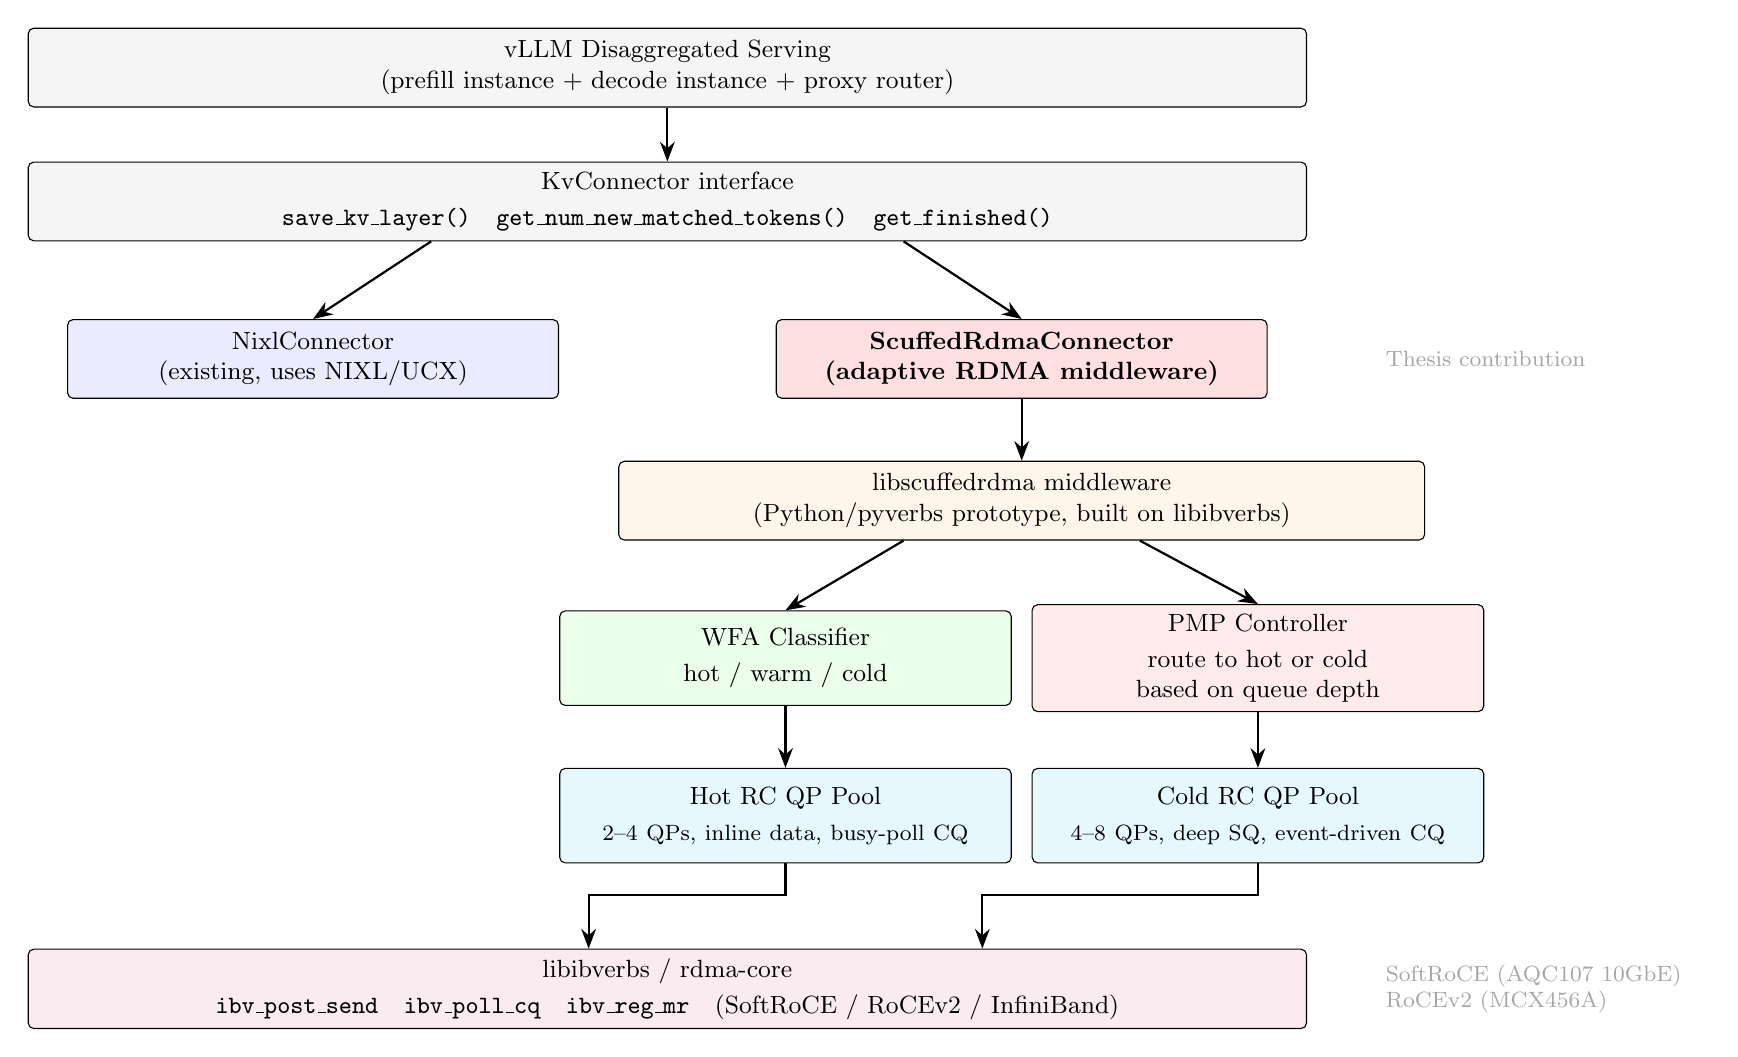
\begin{tikzpicture}[
    layer/.style={rectangle, draw, minimum height=1cm, text centered, font=\small, rounded corners=2pt, text width=#1, align=center},
    layer/.default=10cm,
    thesis/.style={layer=#1, fill=red!12, font=\small\bfseries},
    thesis/.default=5.5cm,
    arr/.style={-{Stealth[length=2.5mm]}, thick}
]

% Row 1: vLLM
\node[layer=16cm, fill=gray!8] (vllm) at (8, 10.5)
    {vLLM Disaggregated Serving\\(prefill instance + decode instance + proxy router)};

% Row 2: KvConnector interface
\node[layer=16cm, fill=gray!8] (kvif) at (8, 8.8)
    {KvConnector interface\\[2pt]\texttt{save\_kv\_layer()}\quad \texttt{get\_num\_new\_matched\_tokens()}\quad \texttt{get\_finished()}};

% Row 3: Connectors side by side
\node[layer=6cm, fill=blue!8] (nixl) at (3.5, 6.8)
    {NixlConnector\\(existing, uses NIXL/UCX)};
\node[thesis=6cm] (scuffed) at (12.5, 6.8)
    {ScuffedRdmaConnector\\(adaptive RDMA middleware)};

% Row 4: libscuffedrdma
\node[layer=10cm, fill=orange!8] (lib) at (12.5, 5)
    {libscuffedrdma middleware\\(Python/pyverbs prototype, built on libibverbs)};

% Row 5: WFA and PMP side by side
\node[layer=5.5cm, fill=green!8, minimum height=1.2cm] (wfa) at (9.5, 3)
    {WFA Classifier\\[2pt]hot / warm / cold};
\node[layer=5.5cm, fill=red!8, minimum height=1.2cm] (pmp) at (15.5, 3)
    {PMP Controller\\[2pt]route to hot or cold based on queue depth};

% Row 6: QP pools
\node[layer=5.5cm, fill=cyan!10, minimum height=1.2cm] (hotqp) at (9.5, 1)
    {Hot RC QP Pool\\[2pt]{\footnotesize 2--4 QPs, inline data, busy-poll CQ}};
\node[layer=5.5cm, fill=cyan!10, minimum height=1.2cm] (coldqp) at (15.5, 1)
    {Cold RC QP Pool\\[2pt]{\footnotesize 4--8 QPs, deep SQ, event-driven CQ}};

% Row 7: Verbs
\node[layer=16cm, fill=purple!8, minimum height=1cm] (verbs) at (8, -1.2)
    {libibverbs / rdma-core\\[2pt]\texttt{ibv\_post\_send}\quad \texttt{ibv\_poll\_cq}\quad \texttt{ibv\_reg\_mr}\quad (SoftRoCE / RoCEv2 / InfiniBand)};

% -- Arrows --
\draw[arr] (vllm) -- (kvif);
\draw[arr] ([xshift=-3cm]kvif.south) -- (nixl.north);
\draw[arr] ([xshift=3cm]kvif.south) -- (scuffed.north);
\draw[arr] (scuffed) -- (lib);
\draw[arr] ([xshift=-1.5cm]lib.south) -- (wfa.north);
\draw[arr] ([xshift=1.5cm]lib.south) -- (pmp.north);
\draw[arr] (wfa) -- (hotqp);
\draw[arr] (pmp) -- (coldqp);
\draw[arr] (hotqp.south) -- ++(0,-0.4) -| ([xshift=-1cm]verbs.north);
\draw[arr] (coldqp.south) -- ++(0,-0.4) -| ([xshift=4cm]verbs.north);

% -- Right-margin annotations (outside diagram, no overlap) --
\node[font=\footnotesize, text=gray!70, anchor=west, text width=4cm] at (17, 6.8)
    {Thesis contribution};
\node[font=\footnotesize, text=gray!70, anchor=west, text width=4cm] at (17, -1.2)
    {SoftRoCE (AQC107 10GbE)\\RoCEv2 (MCX456A)};

\end{tikzpicture}
}
\caption{Full system architecture. The middleware (red) adds tensor-aware classification and priority QP routing on top of UCX/libibverbs, replacing NixlConnector's transport layer. Everything above \texttt{KvConnector} stays stock vLLM.}
\label{fig:full_arch}
\end{figure}

\subsection{The Three API Layers}

\begin{figure}[ht]
\centering
\resizebox{0.92\textwidth}{!}{
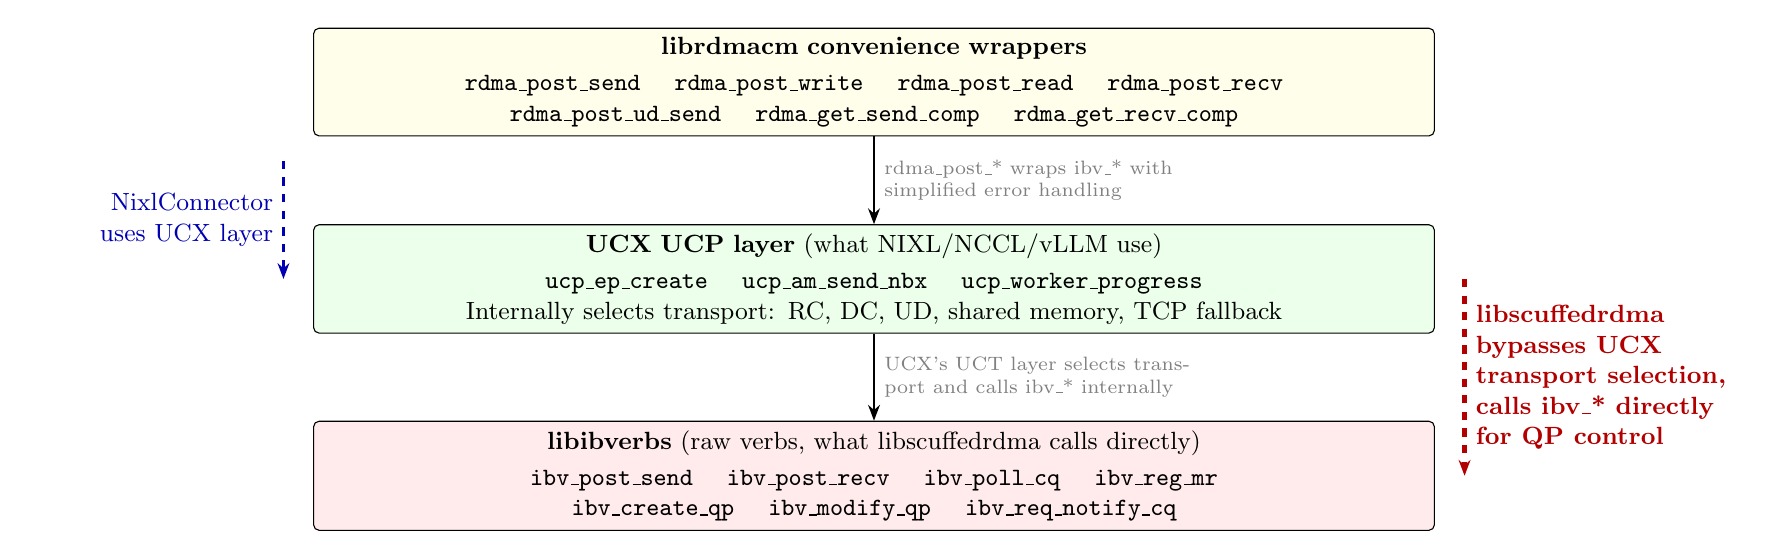
\begin{tikzpicture}[
    box/.style={rectangle, draw, rounded corners=2pt, minimum height=0.9cm, text centered, font=\small, text width=#1, align=center},
    box/.default=5cm,
    arr/.style={-{Stealth[length=2mm]}, thick},
    ann/.style={font=\scriptsize, text=gray}
]

% Layer 1: Convenience (rdma_post_*)
\node[box=14cm, fill=yellow!8] (conv) at (7, 6)
    {\textbf{librdmacm convenience wrappers}\\[2pt]
    \texttt{rdma\_post\_send} \quad \texttt{rdma\_post\_write} \quad \texttt{rdma\_post\_read} \quad \texttt{rdma\_post\_recv}\\
    \texttt{rdma\_post\_ud\_send} \quad \texttt{rdma\_get\_send\_comp} \quad \texttt{rdma\_get\_recv\_comp}};

% Layer 2: UCX UCP
\node[box=14cm, fill=green!8] (ucx) at (7, 3.5)
    {\textbf{UCX UCP layer} (what NIXL/NCCL/vLLM use)\\[2pt]
    \texttt{ucp\_ep\_create} \quad \texttt{ucp\_am\_send\_nbx} \quad \texttt{ucp\_worker\_progress}\\
    Internally selects transport: RC, DC, UD, shared memory, TCP fallback};

% Layer 3: Raw verbs (ibv_*)
\node[box=14cm, fill=red!8] (ibv) at (7, 1)
    {\textbf{libibverbs} (raw verbs, what libscuffedrdma calls directly)\\[2pt]
    \texttt{ibv\_post\_send} \quad \texttt{ibv\_post\_recv} \quad \texttt{ibv\_poll\_cq} \quad \texttt{ibv\_reg\_mr}\\
    \texttt{ibv\_create\_qp} \quad \texttt{ibv\_modify\_qp} \quad \texttt{ibv\_req\_notify\_cq}};

% Arrows
\draw[arr] (conv) -- (ucx) node[midway, right, ann, text width=4cm] {rdma\_post\_* wraps ibv\_* with simplified error handling};
\draw[arr] (ucx) -- (ibv) node[midway, right, ann, text width=4cm] {UCX's UCT layer selects transport and calls ibv\_* internally};

% libscuffedrdma annotation
\draw[arr, color=red!70!black, ultra thick, dashed] (14.5, 3.5) -- (14.5, 1) node[midway, right, font=\small\bfseries, text=red!70!black, text width=3.5cm, align=left] {libscuffedrdma\\bypasses UCX\\transport selection,\\calls ibv\_* directly\\for QP control};

% NixlConnector annotation
\draw[arr, color=blue!70!black, dashed] (-0.5, 5) -- (-0.5, 3.5) node[midway, left, font=\small, text=blue!70!black, text width=3cm, align=right] {NixlConnector\\uses UCX layer};

\end{tikzpicture}
}
\caption{Three RDMA API layers. NixlConnector calls UCX, which internally selects transports. libscuffedrdma bypasses UCX's transport selection and calls \texttt{ibv\_*} directly, which is necessary for controlling which QP each transfer uses.}
\label{fig:api_layers}
\end{figure}

libscuffedrdma bypasses UCX's transport selection and calls \texttt{ibv\_post\_send} directly. UCX routes messages by size alone (small = eager inline send, large = rendezvous RDMA read). This means UCX cannot distinguish between a latency-critical 64KB decode activation and a 64KB background prefetch. libscuffedrdma's WFA classifier makes that distinction, then posts to the correct QP.

The existing vLLM call chain goes: \texttt{save\_kv\_layer()} $\to$ NIXL $\to$ UCX $\to$ \texttt{ibv\_post\_send()}. We replace the middle: \texttt{save\_kv\_layer()} $\to$ WFA classifies $\to$ \texttt{ibv\_post\_send()} on the selected QP.

Both QP pools use RC (Reliable Connected) transport. We do not use UD (Unreliable Datagram) because UD has a 4KB MTU limit requiring application-level fragmentation, no delivery guarantees, and poor SoftRoCE performance. RC handles reliability in hardware. The cost is one QP per peer per priority class, which is trivial for a two-node testbed.

\begin{table}[ht]
\centering\small
\begin{tabular}{lll}
\toprule
& \textbf{Hot Pool (latency)} & \textbf{Cold Pool (throughput)} \\
\midrule
SQ depth & 16 entries & 128 entries \\
CQ depth & 16 entries & 256 entries \\
Inline data & Enabled ($\leq$256B in WR) & Disabled (DMA from MR) \\
CQ polling & Busy-poll, dedicated core & Sleep-poll (event-driven in production) \\
Signaling & Every WR & Every $N$th WR \\
Traffic & KV metadata, heartbeats, all-reduce & Bulk KV blocks, weights, gradients \\
\bottomrule
\end{tabular}
\caption{Hot vs.\ cold RC QP pool configuration. Both pools use RC transport; they differ in tuning.}
\end{table}

\section{Deployment Configurations: Where RDMA Enters the Data Path}

Each configuration below traces four data structures through a distributed LLM inference deployment: \textbf{model weights} (static, loaded once), \textbf{activations} (ephemeral, per-forward-pass), \textbf{KV cache} (grows per-token, persists per-request), and \textbf{control signals} (metadata, scheduling, consensus). The parallelism strategies below follow directly from Austin et al.~\cite{scaling_book} Sections 5 and 7.

\subsection{Configuration A: One User, One Model, Multiple GPUs on One Machine}
\label{sec:config_a}

This is \textbf{tensor parallelism} (TP). Each layer's weight matrices are sharded across GPUs. Every GPU holds a slice of every layer. A single user's request flows through all GPUs at every layer.

\begin{figure}[ht]
\centering
\resizebox{0.85\textwidth}{!}{
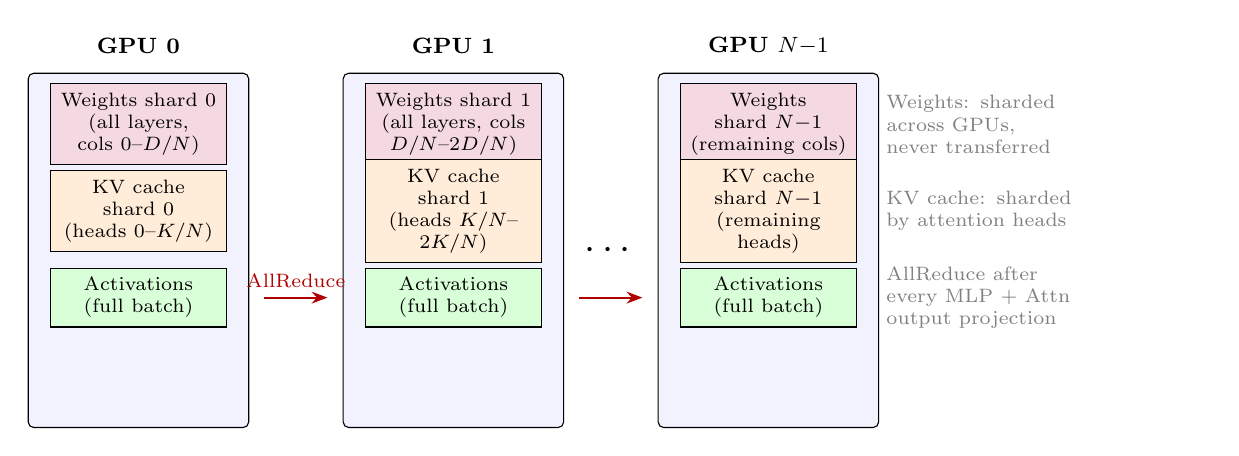
\begin{tikzpicture}[
    gpu/.style={rectangle, draw, rounded corners=2pt, minimum width=2.8cm, minimum height=4.5cm, fill=#1},
    gpu/.default=blue!5,
    wt/.style={rectangle, draw, fill=purple!15, minimum width=2.2cm, minimum height=0.6cm, font=\scriptsize, text width=2cm, align=center},
    kv/.style={rectangle, draw, fill=orange!15, minimum width=2.2cm, minimum height=0.6cm, font=\scriptsize, text width=2cm, align=center},
    act/.style={rectangle, draw, fill=green!15, minimum width=2.2cm, minimum height=0.6cm, font=\scriptsize, text width=2cm, align=center},
    arr/.style={-{Stealth[length=2mm]}, thick},
    lbl/.style={font=\footnotesize\bfseries}
]

\node[gpu] (g0) at (0, 0) {};
\node[lbl] at (0, 2.6) {GPU 0};
\node[wt] at (0, 1.6) {Weights shard 0\\(all layers, cols 0--$D/N$)};
\node[kv] at (0, 0.5) {KV cache shard 0\\(heads 0--$K/N$)};
\node[act] at (0, -0.6) {Activations\\(full batch)};

\node[gpu] (g1) at (4, 0) {};
\node[lbl] at (4, 2.6) {GPU 1};
\node[wt] at (4, 1.6) {Weights shard 1\\(all layers, cols $D/N$--$2D/N$)};
\node[kv] at (4, 0.5) {KV cache shard 1\\(heads $K/N$--$2K/N$)};
\node[act] at (4, -0.6) {Activations\\(full batch)};

\node[gpu] (g2) at (8, 0) {};
\node[lbl] at (8, 2.6) {GPU $N{-}1$};
\node[wt] at (8, 1.6) {Weights shard $N{-}1$\\(remaining cols)};
\node[kv] at (8, 0.5) {KV cache shard $N{-}1$\\(remaining heads)};
\node[act] at (8, -0.6) {Activations\\(full batch)};

\node at (6, 0) {\Large $\cdots$};

% AllReduce arrows
\draw[arr, color=red!70!black] (1.6, -0.6) -- (2.4, -0.6) node[midway, above, font=\scriptsize, text=red!70!black] {AllReduce};
\draw[arr, color=red!70!black] (5.6, -0.6) -- (6.4, -0.6);

% Label
\node[font=\scriptsize, text=gray, text width=4cm, align=left] at (11.5, 1.6) {Weights: sharded\\across GPUs,\\never transferred};
\node[font=\scriptsize, text=gray, text width=4cm, align=left] at (11.5, 0.5) {KV cache: sharded\\by attention heads};
\node[font=\scriptsize, text=gray, text width=4cm, align=left] at (11.5, -0.6) {AllReduce after\\every MLP + Attn\\output projection};

\end{tikzpicture}
}
\caption{\textbf{Config A:} Tensor parallelism, single machine. AllReduce happens over NVLink (intra-node) or PCIe. On consumer hardware without NVLink, PCIe AllReduce is the bottleneck.}
\label{fig:config_a}
\end{figure}

Each GPU computes its shard of the attention and MLP, then AllReduces the partial result with every other GPU. This happens at every layer. The AllReduce messages are small (a few KB to hundreds of KB) but every GPU blocks waiting for them. This is textbook \textbf{hot QP} traffic: small, frequent, latency-critical. On consumer hardware without NVLink, AllReduce goes over PCIe or 10GbE and becomes the bottleneck. When GPU IPC is unavailable, vLLM falls back to NCCL for inter-node AllReduce, which is where libscuffedrdma enters.

\subsection{Configuration B: Multiple Users, One Model, One Machine}

Same as Config A but with continuous batching ($B > 1$ users). Each user has their own KV cache, so total KV memory per GPU scales as $B \times L \times 2 \times K \times H / N$. The RDMA traffic is the same (AllReduce on hot QP) but payloads grow with batch size.

\begin{figure}[ht]
\centering
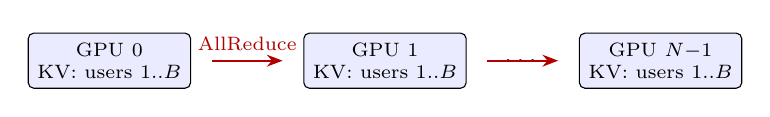
\begin{tikzpicture}[
    box/.style={rectangle, draw, rounded corners=2pt, fill=#1, minimum width=2cm, minimum height=0.7cm, font=\scriptsize, align=center},
    arr/.style={-{Stealth[length=2mm]}, thick}
]
\node[box=blue!8] (g0) at (0,0) {GPU 0\\KV: users 1..$B$};
\node[box=blue!8] (g1) at (3.5,0) {GPU 1\\KV: users 1..$B$};
\node[box=blue!8] (g2) at (7,0) {GPU $N{-}1$\\KV: users 1..$B$};
\node at (5.25,0) {\dots};
\draw[arr, color=red!70!black] (1.3,0) -- (2.2,0) node[midway, above, font=\scriptsize, text=red!70!black] {AllReduce};
\draw[arr, color=red!70!black] (4.8,0) -- (5.7,0);
\end{tikzpicture}
\caption{\textbf{Config B:} Tensor parallelism with continuous batching. Each GPU holds KV caches for all $B$ concurrent users. AllReduce traffic matches Config A but KV memory scales with batch size.}
\end{figure}

\subsection{Configuration C: Disaggregated Prefill/Decode Across Machines}
\label{sec:config_c}

This is the primary target of the thesis. Prefill and decode run on \textbf{separate machines}. The prefill node processes the full prompt and generates the KV cache. The prefill node then transfers the KV cache over the network to the decode node, which generates tokens autoregressively.

\begin{figure}[ht]
\centering
\resizebox{0.95\textwidth}{!}{
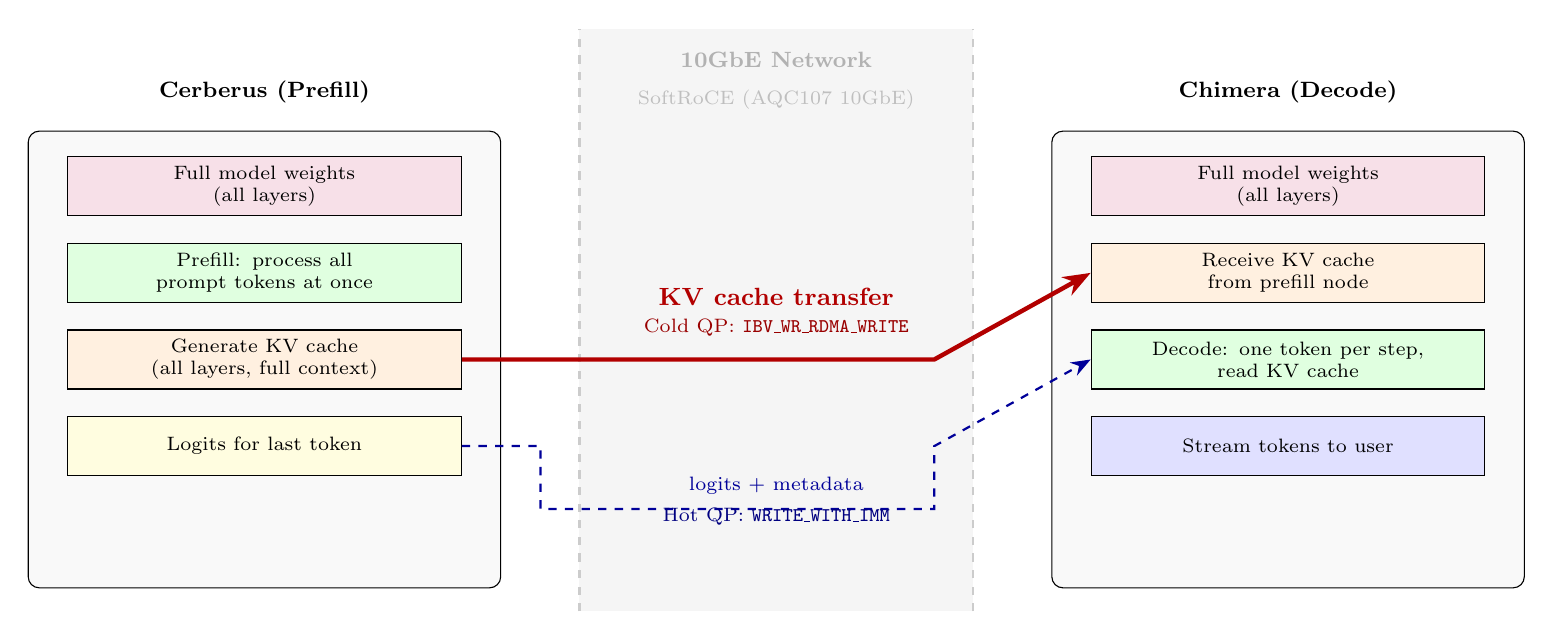
\begin{tikzpicture}[
    machine/.style={rectangle, draw, rounded corners=4pt, minimum width=6cm, minimum height=5.8cm, fill=gray!5},
    comp/.style={rectangle, draw, fill=#1, minimum width=5cm, minimum height=0.75cm, font=\scriptsize, align=center, text width=4.5cm},
    comp/.default=white,
    arr/.style={-{Stealth[length=2.5mm]}, thick},
    bigarr/.style={-{Stealth[length=3.5mm]}, ultra thick, color=red!70!black},
    lbl/.style={font=\footnotesize\bfseries}
]

% Prefill machine (left)
\node[machine] (m1) at (0, 0) {};
\node[lbl] at (0, 3.4) {Cerberus (Prefill)};
\node[comp=purple!12] (pw) at (0, 2.2) {Full model weights\\(all layers)};
\node[comp=green!12] (pa) at (0, 1.1) {Prefill: process all\\prompt tokens at once};
\node[comp=orange!12] (pkv) at (0, 0.0) {Generate KV cache\\(all layers, full context)};
\node[comp=yellow!12] (pl) at (0, -1.1) {Logits for last token};

% Decode machine (right, wider gap)
\node[machine] (m2) at (13, 0) {};
\node[lbl] at (13, 3.4) {Chimera (Decode)};
\node[comp=purple!12] (dw) at (13, 2.2) {Full model weights\\(all layers)};
\node[comp=orange!12] (dkv) at (13, 1.1) {Receive KV cache\\from prefill node};
\node[comp=green!12] (da) at (13, 0.0) {Decode: one token per step,\\read KV cache};
\node[comp=blue!12] (do) at (13, -1.1) {Stream tokens to user};

% Network zone (shaded strip between machines)
\fill[gray!8] (4, -3.2) rectangle (9, 4.2);
\draw[thick, gray!40, dashed] (4, -3.2) -- (4, 4.2);
\draw[thick, gray!40, dashed] (9, -3.2) -- (9, 4.2);
\node[font=\footnotesize\bfseries, text=gray!60] at (6.5, 3.8) {10GbE Network};
\node[font=\scriptsize, text=gray!50] at (6.5, 3.3) {SoftRoCE (AQC107 10GbE)};

% KV cache transfer (top arrow through network zone)
\draw[bigarr] (pkv.east) -- ++(1, 0) -- ++(5, 0) -- (dkv.west);
\node[font=\small\bfseries, text=red!70!black] at (6.5, 0.8) {KV cache transfer};
\node[font=\scriptsize, text=red!60!black] at (6.5, 0.4) {Cold QP: \texttt{IBV\_WR\_RDMA\_WRITE}};

% Logits + metadata (bottom arrow, dashed, shifted down to avoid overlap)
\draw[arr, dashed, color=blue!60!black] (pl.east) -- ++(1, 0) -- ++(0, -0.8) -- ++(5, 0) -- ++(0, 0.8) -- (da.west);
\node[font=\scriptsize, text=blue!60!black] at (6.5, -1.6) {logits + metadata};
\node[font=\scriptsize, text=blue!50!black] at (6.5, -2.0) {Hot QP: \texttt{WRITE\_WITH\_IMM}};

\end{tikzpicture}
}
\caption{\textbf{Config C:} Disaggregated prefill/decode. The thick red arrow is the critical-path RDMA transfer that determines TTFT. The dashed blue arrow carries latency-sensitive metadata on the hot QP.}
\label{fig:config_c}
\end{figure}

\paragraph{Data flow.}
The prefill node processes the full prompt in one compute-bound forward pass, producing the KV cache for all layers and the logits for the last token. Both are transferred to the decode node via RDMA. The decode node holds its own copy of model weights, receives the KV cache, and generates tokens autoregressively (memory-bandwidth-bound), appending one token's KV per step.

\paragraph{What crosses the network.}
The KV cache is the dominant transfer. For a model with $L$ layers, $K$ KV heads, head dimension $H$, and sequence length $S$:
\[
\text{KV transfer size} = 2 \times \text{bytes} \times H \times K \times L \times S
\]
The logits and request metadata are small (a few KB). On 10GbE, the KV transfer is the TTFT bottleneck.

\paragraph{Dual QP mapping.}
\textbf{Hot QP:} logits, request metadata, scheduling signals, and consensus heartbeats if a protocol like Raft were added for multi-node coordination. These are small and latency-critical: the decode node cannot begin until it has the logits. \textbf{Cold QP:} bulk KV cache blocks. These are large but can be pipelined layer-by-layer (TransferEngine pattern~\cite{chen2025transferengine}). The cold QP uses \texttt{IBV\_WR\_RDMA\_WRITE} for zero-copy one-sided transfers from prefill GPU memory to decode GPU memory. With GPUDirect RDMA, this is truly zero-copy; on Cerberus/Chimera with SoftRoCE, data stages through host memory.

\paragraph{Compression reduces the cold QP load.}
LoRC~\cite{zhang2024lorc} reduces $H$ (lower-dimensional KV vectors). KVTC~\cite{kvtc2024} applies entropy coding on the KV tensors. TurboQuant~\cite{turboquant2026} reduces bytes-per-element. Each shrinks the cold QP payload, but the hot QP traffic (metadata, logits) is unaffected since it is already small.

\subsection{Configuration D: Multiple Users, One Model, Multiple Machines}

This combines Configs B and C: disaggregated prefill/decode with continuous batching across multiple users.

\begin{figure}[ht]
\centering
\resizebox{0.92\textwidth}{!}{
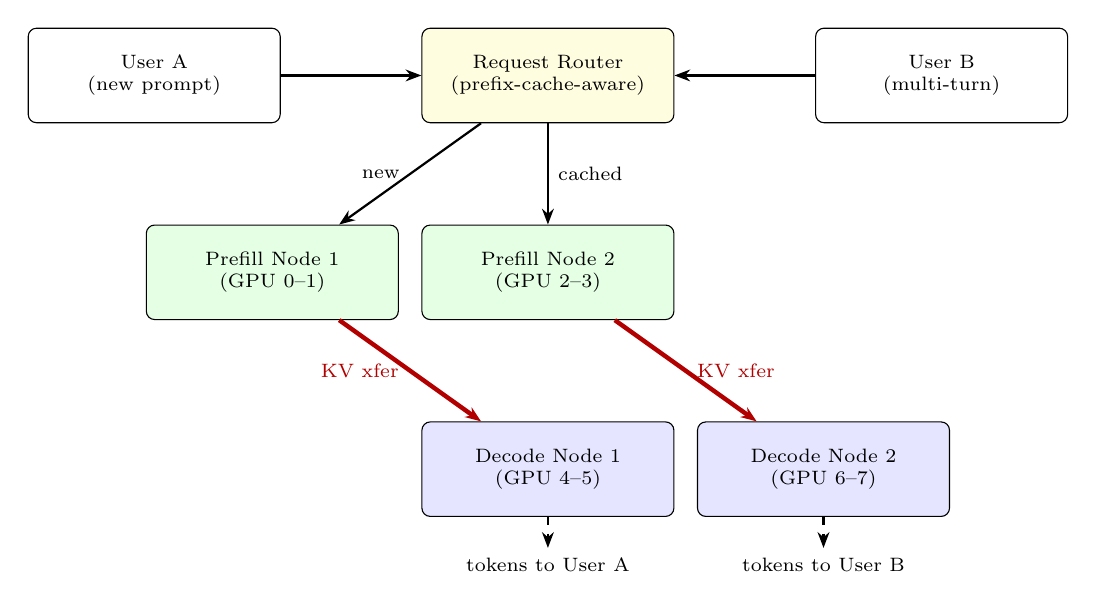
\begin{tikzpicture}[
    node/.style={rectangle, draw, rounded corners=3pt, minimum width=3.2cm, minimum height=1.2cm, fill=#1, font=\scriptsize, align=center, text width=2.8cm},
    node/.default=gray!8,
    arr/.style={-{Stealth[length=2mm]}, thick},
    lbl/.style={font=\footnotesize\bfseries}
]

% Router
\node[node=yellow!12] (router) at (5, 5) {Request Router\\(prefix-cache-aware)};

% Users
\node[node=white] (u1) at (0, 5) {User A\\(new prompt)};
\node[node=white] (u2) at (10, 5) {User B\\(multi-turn)};

% Prefill pool
\node[node=green!10] (p1) at (1.5, 2.5) {Prefill Node 1\\(GPU 0--1)};
\node[node=green!10] (p2) at (5, 2.5) {Prefill Node 2\\(GPU 2--3)};

% Decode pool
\node[node=blue!10] (d1) at (5, 0) {Decode Node 1\\(GPU 4--5)};
\node[node=blue!10] (d2) at (8.5, 0) {Decode Node 2\\(GPU 6--7)};

% Arrows
\draw[arr] (u1) -- (router);
\draw[arr] (u2) -- (router);
\draw[arr] (router) -- (p1) node[midway, left, font=\scriptsize] {new};
\draw[arr] (router) -- (p2) node[midway, right, font=\scriptsize] {cached};
\draw[arr, color=red!70!black, ultra thick] (p1) -- (d1) node[midway, left, font=\scriptsize, text=red!70!black] {KV xfer};
\draw[arr, color=red!70!black, ultra thick] (p2) -- (d2) node[midway, right, font=\scriptsize, text=red!70!black] {KV xfer};
\draw[arr, dashed] (d1) -- ++(0, -1) node[below, font=\scriptsize] {tokens to User A};
\draw[arr, dashed] (d2) -- ++(0, -1) node[below, font=\scriptsize] {tokens to User B};

\end{tikzpicture}
}
\caption{\textbf{Config D:} Multi-user disaggregated serving. The router directs requests to prefill nodes based on prefix cache locality (llm-d pattern~\cite{llmd_v05}). KV transfers (red) are independent per-user and can be multiplexed on the same link.}
\label{fig:config_d}
\end{figure}

Multiple users' KV transfers share the same 10GbE link. Without traffic separation, User A's large KV transfer blocks User B's small metadata. That's the head-of-line blocking problem the dual QP pool solves. The PMP controller allocates bandwidth between pools based on queue depth. With prefix caching (llm-d~\cite{llmd_v05}), some KV blocks are already on the decode node, which changes the traffic pattern the WFA observes.

\subsection{Configuration E: Multiple Models, Multiple Machines}

MoE (Mixture-of-Experts) models and multi-model serving.

\begin{figure}[ht]
\centering
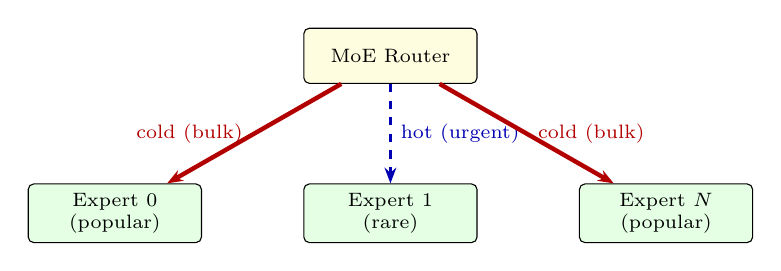
\begin{tikzpicture}[
    box/.style={rectangle, draw, rounded corners=2pt, fill=#1, minimum width=2.2cm, minimum height=0.7cm, font=\scriptsize, align=center},
    arr/.style={-{Stealth[length=2mm]}, thick}
]
\node[box=yellow!12] (router) at (3.5,2) {MoE Router};
\node[box=green!10] (e0) at (0,0) {Expert 0\\(popular)};
\node[box=green!10] (e1) at (3.5,0) {Expert 1\\(rare)};
\node[box=green!10] (e2) at (7,0) {Expert $N$\\(popular)};
\draw[arr, color=red!70!black, ultra thick] (router) -- (e0) node[midway, left, font=\scriptsize, text=red!70!black] {cold (bulk)};
\draw[arr, color=blue!70!black, dashed] (router) -- (e1) node[midway, right, font=\scriptsize, text=blue!70!black] {hot (urgent)};
\draw[arr, color=red!70!black, ultra thick] (router) -- (e2) node[midway, right, font=\scriptsize, text=red!70!black] {cold (bulk)};
\end{tikzpicture}
\caption{\textbf{Config E:} MoE expert parallelism. Popular experts get large batches (cold QP), rare experts get small urgent transfers (hot QP).}
\end{figure}

In MoE models (e.g. DeepSeek-V3), each token routes to a subset of experts across machines, creating All-to-All traffic at every layer. Popular experts get large predictable batches (cold QP), rare experts get small urgent transfers (hot QP). The WFA classifies by per-expert access frequency. vLLM's elastic expert parallelism (PR \#34861~\cite{vllm_pr34861}) produces this same hot/cold split when GPUs are dynamically added or removed.

\subsection{Summary: QP and Verbs Mapping by Configuration}

\begin{table}[ht]
\centering\small
\begin{tabular}{llll}
\toprule
\textbf{Config} & \textbf{Hot QP traffic} & \textbf{Cold QP traffic} & \textbf{Primary verb} \\
\midrule
A: TP, 1 user, 1 machine & AllReduce fragments & (none) & \texttt{WRITE\_WITH\_IMM} \\
B: TP, $N$ users, 1 machine & AllReduce fragments & (none) & \texttt{WRITE\_WITH\_IMM} \\
C: Disagg P/D, 1 user & Logits, metadata & KV cache blocks & \texttt{WRITE} (cold) \\
D: Disagg P/D, $N$ users & Metadata, scheduling & Multiplexed KV & \texttt{WRITE} (cold) \\
E: MoE / multi-model & Rare expert tokens & Popular expert tokens & \texttt{WRITE\_WITH\_IMM} \\
\bottomrule
\end{tabular}
\caption{QP and verbs mapping by deployment configuration. Config C is the thesis's primary target; Configs D and E are stretch goals.}
\label{tab:config_summary}
\end{table}

\paragraph{What to optimize first.}
Config C (disaggregated prefill/decode, single user) is the simplest configuration that exercises the full dual QP architecture. It has a clear hot/cold separation (metadata vs.\ KV blocks), a measurable TTFT metric, and maps directly onto the Cerberus/Chimera testbed. Once Config C works, extending to Config D (multiple users) adds the multiplexing problem that makes the PMP controller's bang-bang allocation necessary. Config E (MoE) is the most complex but produces the richest WFA training data due to the bimodal expert access pattern.

\section{UCX Issue Landscape and Upstream Contributions}

UCX is the dominant open-source RDMA transport framework. NCCL, MPI, PyTorch, and Dask all use it. While building libscuffedrdma we ran into recurring architectural issues in UCX's issue tracker, and ended up contributing six fixes upstream. This section covers the problems we hit, the bypass we built in libscuffedrdma, and the patches we sent to UCX.

\subsection{Problems Identified}

UCX makes three design choices that create friction for LLM inference workloads:

\begin{enumerate}
    \item \textbf{Size-only routing.} Messages below \texttt{UCX\_RNDV\_THRESH} take the eager path; messages above take rendezvous. This creates latency cliffs at the threshold and cannot distinguish a latency-critical decode transfer from a background prefetch of the same size (Issues \#10552, \#10486, \#10532, \#4430, \#11091).

    \item \textbf{Shared QP pools.} All traffic shares the same QPs, so a small message can queue behind a large transfer. Processes share UDP source ports (breaking bond hashing, \#11004), contend on spinlocks (\#11034), and cannot defer QP allocation (\#1319).

    \item \textbf{Opaque transport selection.} Users cannot inspect, override, or query which transport UCX chose (\#10652, \#6511, \#9364, \#10608). Multi-rail often degrades performance instead of improving it (\#9520, \#10669, \#10420). The rendezvous path has open bugs since 2017 (\#6721, \#10568, \#1298--\#1300).
\end{enumerate}

Additional friction for ML workloads includes silent memory registration failures (\#7989), 25--75\% TCP slowdown when CUDA is compiled in (\#7880), and asymmetric traffic class application (\#10325).

\subsection{libscuffedrdma's Response}

libscuffedrdma bypasses UCX's data path entirely. Instead of size-based routing through shared QPs, the WFA classifier assigns each transfer a priority class based on tensor metadata (access frequency, inference phase, layer index), and the PMP controller routes it to a dedicated hot or cold QP. All data-path calls go through \texttt{ibv\_post\_send} directly with pre-registered memory regions. The mapping from tensor to QP is deterministic: there's no opaque scoring or rendezvous handshake, and the hot and cold pools don't share QPs.

Table~\ref{tab:ucx_issue_map} maps each libscuffedrdma component to the UCX issues it addresses.

\begin{table}[ht]
\centering\small
\begin{tabular}{@{}p{4.2cm}p{3.0cm}p{5.5cm}@{}}
\toprule
\textbf{Component} & \textbf{UCX Issues} & \textbf{What It Does} \\
\midrule
WFA classifier & \#10552, \#10486, \#10532, \#4430, \#11091 & Replaces size-only threshold with tensor metadata classification \\
\addlinespace
Hot/cold QP pools & \#11004, \#11034, \#1319 & Dedicated QPs per traffic class eliminate head-of-line blocking \\
\addlinespace
Direct \texttt{ibv\_post\_send} & \#6721, \#10568, \#3542, \#1298--\#1300 & Bypasses rendezvous handshake, rail selection, and wakeup overhead \\
\addlinespace
Pre-registered MRs & \#10719, \#7989, \#6264 & One-time \texttt{ibv\_reg\_mr} at startup with explicit error handling \\
\addlinespace
PMP controller & \#9520, \#10669 & Control-theoretic QP allocation replaces static lane scoring \\
\addlinespace
Per-QP traffic class & \#11252, \#10325 & Symmetric TC via direct \texttt{ibv\_modify\_qp} on both endpoints \\
\bottomrule
\end{tabular}
\caption{libscuffedrdma components mapped to the UCX issues they address.}
\label{tab:ucx_issue_map}
\end{table}

\subsection{Upstream UCX Contributions}

Beyond the bypass, we submitted six pull requests to \texttt{openucx/ucx} that fix the issues directly (Table~\ref{tab:ucx_prs}).

\begin{table}[ht]
\centering\small
\begin{tabular}{@{}llp{7.8cm}@{}}
\toprule
\textbf{PR} & \textbf{Fixes} & \textbf{Change} \\
\midrule
\href{https://github.com/openucx/ucx/pull/11304}{\#11304} & \#4430 & Use calculated RNDV threshold for \texttt{ucp\_tag\_send\_nbr()} instead of hardcoded 256KB \\
\addlinespace
\href{https://github.com/openucx/ucx/pull/11305}{\#11305} & \#1307 & Adaptive TX CQ moderation: force signaled send when CQ credits run low to prevent TX stalls \\
\addlinespace
\href{https://github.com/openucx/ucx/pull/11306}{\#11306} & \#4275 & Allow eager inline sends for host memory when CUDA memory domains are loaded \\
\addlinespace
\href{https://github.com/openucx/ucx/pull/11307}{\#11307} & \#4794 & Add TCP as fallback wireup transport for RC/DC on SoftRoCE where UD is unavailable \\
\addlinespace
\href{https://github.com/openucx/ucx/pull/11308}{\#11308} & \#6254 & Add \texttt{ucp\_ep\_query()} bandwidth estimate for informed application placement decisions \\
\addlinespace
\href{https://github.com/openucx/ucx/pull/11309}{\#11309} & \#10325 & Propagate traffic class in IB address for symmetric QoS on both connection directions \\
\bottomrule
\end{tabular}
\caption{Upstream UCX pull requests submitted to \texttt{openucx/ucx} on GitHub.}
\label{tab:ucx_prs}
\end{table}

\section{KV Cache Compression Pipeline and TurboQuant}

\subsection{Three Compression Stages on Orthogonal Axes}

\textbf{LoRC}~\cite{zhang2024lorc} applies SVD to $W_K, W_V$, producing lower-dimensional KV vectors at every forward pass without retraining. The progressive strategy retains more singular values in shallow layers (sensitive to truncation) and compresses deep layers aggressively. Zhang et al.\ report significant compression with negligible quality degradation across LLaMA-8B through 70B~\cite{zhang2024lorc}. Whether this improves TTFT on our testbed is untested.

LoRC, KVTC~\cite{kvtc2024}, and TurboQuant~\cite{turboquant2026} target orthogonal representation axes and compose as a pipeline. The pipeline for a KV vector $k \in \mathbb{R}^d$ is:
\[
k \xrightarrow{\text{LoRC (dim)}} k' \in \mathbb{R}^{d'} \xrightarrow{\text{KVTC (redundancy)}} \tilde{k} \in \mathbb{R}^{d'} \xrightarrow{\text{TurboQuant (precision)}} \hat{k} \in \{0,\ldots,2^b-1\}^{d'}
\]
LoRC reduces $d \to d'$ via SVD on the weight matrices. KVTC applies PCA decorrelation and entropy coding on the generated vectors. TurboQuant reduces the bits-per-element from 16 to as low as 3 while preserving inner product accuracy. Because each stage operates on a different axis of the representation, their effects compound.

\subsection{TurboQuant}

TurboQuant~\cite{turboquant2026} (Zandieh, Mirrokni et al., Google Research) is a two-stage quantization algorithm that does not need per-block calibration data:

\begin{enumerate}
\item \textbf{PolarQuant}: Apply a random rotation to the KV vector, then quantize. The rotation makes each coordinate's distribution predictable, so the quantizer can be pre-computed once and reused for all vectors. No per-block normalization constants needed.
\item \textbf{QJL correction}: The quantization error creates bias in inner products. TurboQuant corrects this by storing a 1-bit sketch of the residual using the Quantized Johnson-Lindenstrauss transform. The corrected inner products are provably unbiased.
\end{enumerate}

The key detail for RDMA: TurboQuant preserves \emph{inner product accuracy}, not individual vector accuracy. Attention only needs inner products (query dot key), so this works, but the decode node needs a modified attention kernel that operates on the quantized codes directly. The RDMA layer just moves the smaller compressed bytes.

\subsection{How Compression and Transport Interact}

Compression (TurboQuant, KVTC, LoRC) reduces the bytes that cross the link. The dual QP pool reduces the queuing delay on the link. These target different terms:
\[
T_{\text{KV transfer}} = \underbrace{\frac{\text{KV}_{\text{bytes}}}{W_{\text{net}}}}_{\text{compression reduces this}} + \underbrace{T_{\text{queuing delay}}}_{\text{dual QP reduces this}}
\]
The RDMA layer is agnostic to whether bytes are compressed. The WFA classifies by size and access pattern, not data content. However, compression shifts the size distribution: blocks that were ``large'' (cold path) may become ``small'' (hot path) after compression, so the WFA thresholds should be tuned on compressed traffic.

KVTC (NVIDIA) requires per-model calibration but achieves higher compression. TurboQuant (Google) is model-independent but compresses less. They target different pipeline stages and can be combined. The RDMA transport work is independent of both.

\section{Production Systems Context}

\textbf{NVIDIA Dynamo/NIXL}~\cite{nvidia_dynamo2025}: NIXL selects backends automatically but lacks adaptive QP management. libscuffedrdma fills this gap.

\textbf{llm-d v0.5}~\cite{llmd_v05}: UCCL's software transport with fine-grained flow splitting provides greater congestion resilience than UCX~\cite{nvidia_ucx} by avoiding hardware PFC. Their prefix-cache-aware scheduling reduces TTFT by routing to nodes holding the relevant KV cache.

\textbf{TransferEngine}~\cite{chen2025transferengine}: Bridges common NICs to expose a uniform interface for point-to-point RDMA in LLM systems, implementing one-sided WriteImm operations across multiple NICs per GPU. libscuffedrdma extends this with tensor-aware classification for QP selection.

\textbf{Consensus protocols}~\cite{paxos_raft_zab}: If a consensus layer (e.g. Raft) were added, heartbeats would be a textbook hot-path case. On a single 10GbE NIC, a heartbeat blocked behind a large KV transfer could trigger spurious leader elections. No consensus protocol is implemented yet; this is a planned extension.

\textbf{Consumer network roofline}~\cite{scaling_book}: On 10GbE ($\sim$1.2 GB/s), operations that are compute-bound in datacenters (all-reduce, KV transfer) become communication-bound. Software RDMA optimization yields larger relative gains on consumer hardware, where bandwidth is scarce and inefficiencies cannot be masked by raw throughput.



\section{Benchmark Results}

The following results were collected on Chimera (3$\times$ RTX 3090, Aquantia AQC107 10GbE, SoftRoCE/rxe0, Ubuntu 24.04, CUDA 12.4, Python 3.12, pyverbs 50.0). All measurements use real RDMA Write operations over the rxe kernel driver.

\subsection{Dual QP Pool: Head-of-Line Blocking}

\begin{table}[h]
\centering
\caption{Small-transfer latency under mixed 256B + 1MB workload (1000 iterations, SoftRoCE loopback).}
\label{tab:dual_qp_results}
\begin{tabular}{lrrr}
\toprule
Scenario & p50 ($\mu$s) & p95 ($\mu$s) & p99 ($\mu$s) \\
\midrule
Single QP (baseline) & 13.6 & 15.9 & 17.7 \\
Dual QP (WFA classifier) & 14.2 & 17.7 & 21.4 \\
Dual QP + PMP controller & 14.5 & 18.5 & 23.2 \\
\bottomrule
\end{tabular}
\end{table}

The dual QP scenarios are 0.5--5.5$\mu$s slower than the single QP baseline (p50 to p99, PMP enabled). This is expected:

\paragraph{Why dual QP is slower here.} SoftRoCE is synchronous and single-threaded: transfers execute one at a time, so no head-of-line blocking occurs. The overhead comes from managing two pools instead of one: round-robin QP selection, building separate GlobalRoute and AHAttr structures per QP, running the WFA classifier (access count lookup, phase detection, threshold checks), and running the PMP controller (switching function, history tracking).

\paragraph{Why this changes with real hardware.} SoftRoCE implements RDMA in the kernel: the CPU handles QP state transitions, packet construction, and completions in software. On hardware (e.g., ConnectX-6), the NIC processes the send queue and generates completions without CPU involvement. This changes two things:

\begin{itemize}
\item \textbf{Base latency drops.} Hardware RDMA on ConnectX typically achieves 1--2$\mu$s for small messages vs our 13--14$\mu$s on SoftRoCE. The measured dual-QP overhead (0.5--5.5$\mu$s, including classification, routing, and PMP) becomes a larger fraction of the transfer time but is still small relative to the cold path.
\item \textbf{QP isolation becomes real.} With hardware offload, the NIC processes each QP's send queue independently. A 1MB write occupying the cold QP does not block the hot QP because the NIC has separate hardware contexts for each. With SoftRoCE, the kernel processes everything sequentially regardless of which QP it belongs to. Hardware RDMA is where the dual QP architecture pays off: concurrent producers can post to hot and cold QPs simultaneously, and the NIC drains them in parallel.
\end{itemize}

\paragraph{When head-of-line blocking appears.} The benefit requires at least one of: (a) multiple threads posting transfers concurrently, so one thread's 1MB cold write is in-flight while another thread's 256B hot write needs to go out; or (b) async posting with queue depth $> 0$, where multiple work requests are queued before any complete. In both cases, sharing a single QP means the 256B message waits behind the 1MB message in the send queue. Separate QPs eliminate this wait. The concurrent workload benchmark and cross-node testing on real hardware are the next steps to measure this.

\subsection{Latency Across Message Sizes}

\begin{table}[h]
\centering
\caption{libscuffedrdma latency vs.\ message size (50 iterations per size, SoftRoCE loopback). Sizes marked $\dag$ correspond to UCX eager/RNDV protocol transition boundaries.}
\label{tab:ucx_comparison}
\begin{tabular}{rrrrl}
\toprule
Size (B) & p50 ($\mu$s) & p95 ($\mu$s) & p99 ($\mu$s) & Pool \\
\midrule
64 & 12.6 & 19.4 & 48.1 & hot \\
256 & 12.9 & 14.2 & 24.6 & hot \\
1024 & 12.8 & 13.6 & 24.8 & hot \\
3000$^\dag$ & 18.7 & 22.4 & 30.8 & hot \\
8192$^\dag$ & 32.7 & 41.3 & 44.5 & hot \\
32768$^\dag$ & 98.4 & 110.6 & 112.8 & hot \\
65536$^\dag$ & 183.8 & 206.4 & 278.2 & hot \\
262144 & 704.9 & 732.4 & 742.3 & hot \\
524288 & 1414.5 & 1450.4 & 1459.1 & cold \\
1048576 & 2822.6 & 2863.6 & 3104.0 & cold \\
\bottomrule
\end{tabular}
\end{table}

The latency curve is smooth and monotonic across all message sizes. There is no cliff at the 8KB, 30KB, 32KB, or 64KB boundaries where UCX switches between eager, zcopy, and rendezvous protocols (issues \#10552, \#10486, \#10532). The WFA classifier switches from hot to cold at 512KB. The configured size threshold is 256KB, but frequently-accessed tensors get promoted to hot, pushing the effective crossover to 512KB.

\subsection{Infrastructure Validation}

\begin{table}[h]
\centering
\caption{Chimera infrastructure state (March 2026).}
\label{tab:infra}
\begin{tabular}{ll}
\toprule
Component & Status \\
\midrule
RDMA device & rxe0 ACTIVE on enp69s0 (10Gbps, MTU 9000) \\
GPUs & 3$\times$ NVIDIA GeForce RTX 3090 \\
CUDA & 12.4.131 \\
UCX & 1.16.0 (verbs, mlx5-dv, RC, DC, UD) \\
nvidia-peermem & Available (v550.144.03), not loaded \\
NIC & Aquantia AQC107 10GbE \\
Python / pyverbs & 3.12.3 / 50.0 \\
\bottomrule
\end{tabular}
\end{table}

\section{Implementation: Python MVP on SoftRoCE}

The Python implementation validates the dual QP architecture on real RDMA hardware before porting to C++. All code uses pyverbs (Python bindings for rdma-core) against the SoftRoCE kernel driver (\texttt{rdma\_rxe}) on Chimera's Aquantia AQC107 10GbE NIC.

\subsection{RDMA Connection Lifecycle}

Every RDMA transfer requires a connected queue pair (QP). A QP starts in RESET state and must transition through three states before it can send data. Both sides must go through these transitions. Before connecting, they swap QP numbers and GIDs over a separate TCP connection (RDMA has no discovery mechanism).

\begin{verbatim}
  SETUP:
    ctx = open_device("rxe0")
    pd  = alloc_protection_domain(ctx)
    cq  = create_completion_queue(ctx, depth)
    qp  = create_queue_pair(pd, cq, type=RC)

  CONNECT (both sides, with remote info exchanged over TCP):
    qp.to_init(port=1, access=LOCAL_WRITE|REMOTE_WRITE|REMOTE_READ)
    qp.to_rtr(remote_qpn, remote_gid, mtu=1024)
    qp.to_rts(timeout=14, retry=7)

  REGISTER MEMORY:
    mr = register_region(pd, size, access=LOCAL_WRITE|REMOTE_WRITE)
    -- mr.buf is the virtual address, mr.lkey/rkey are access keys

  TRANSFER (one-sided, no remote CPU involvement):
    post_send(qp, opcode=RDMA_WRITE, local_buf, remote_addr, remote_rkey)
    poll_cq(cq) -- blocks until NIC confirms completion
\end{verbatim}

The key insight: \texttt{RDMA\_WRITE} writes directly into remote memory using the remote address and rkey. The remote CPU never sees the transfer. This is what makes RDMA fast, and why QP isolation matters: if hot and cold traffic share a QP, the NIC processes them in FIFO order.

\subsection{Dual QP Pool}

The \texttt{DualQPPool} class creates two separate pools of QPs on the same protection domain. Each pool has its own completion queues, so polling one pool never touches the other.

\begin{verbatim}
  class DualQPPool:
    open():
      ctx = open_device("rxe0")
      pd  = alloc_protection_domain(ctx)
      gid = query_gid(port=1, index=1)  -- link-local IPv6

      for i in 0..n_hot:
        hot_qps[i] = create_qp(pd, cq_depth=16,  max_send=16)
      for i in 0..n_cold:
        cold_qps[i] = create_qp(pd, cq_depth=256, max_send=128)

    post_write_hot(buf, remote_addr, remote_rkey, length):
      qp = hot_qps[round_robin++ % n_hot]
      t0 = now()
      post_rdma_write(qp, buf, remote_addr, remote_rkey, length)
      busy_poll(qp.cq)           -- spin until completion
      return (now() - t0) in microseconds

    post_write_cold(buf, remote_addr, remote_rkey, length):
      qp = cold_qps[round_robin++ % n_cold]
      t0 = now()
      post_rdma_write(qp, buf, remote_addr, remote_rkey, length)
      sleep_poll(qp.cq, 50us)   -- poll, sleep 50us, repeat
      return (now() - t0) in microseconds
\end{verbatim}

Hot QPs busy-poll (spin on the CQ until a completion arrives). This burns CPU but gives minimum latency. Cold QPs sleep-poll (check, sleep 50$\mu$s, check again). This frees CPU for other work at the cost of up to 50$\mu$s added latency per poll cycle.

\subsection{WFA Classifier}

The classifier decides which pool handles each transfer. It examines three things: transfer size, access frequency, and inference phase.

\begin{verbatim}
  classify(tensor_id, size_bytes, layer_idx):
    count = increment_access_count(tensor_id)
    phase = detect_phase(layer_idx)

    -- Size routing (primary decision)
    if size < 4KB:       queue = HOT
    elif size > 256KB:   queue = COLD
    else:
      if count >= 10:    queue = HOT    -- frequently accessed
      else:              queue = COLD   -- infrequent

    -- Phase adjustment
    if phase == PREFILL and queue == HOT and size > 2KB:
      queue = COLD       -- prefill is bulk, bias cold
    if phase == DECODE and queue == COLD and count >= 5:
      queue = HOT        -- decode is latency-sensitive, bias hot

    return queue

  detect_phase(layer_idx):
    recent = last 8 layer indices seen
    if recent == [L, L+1, L+2, ...]:  return PREFILL
    if recent == [L, L, L, ...]:      return DECODE
    else:                              return UNKNOWN
\end{verbatim}

Phase detection works by observing layer access order. Prefill sweeps sequentially through all layers (L0, L1, L2, ...). Decode repeatedly accesses the same layer as it generates tokens. The classifier figures out the phase on its own, so the inference engine doesn't have to signal it.

\subsection{PMP Bang-Bang Controller}

The controller monitors queue depths and overrides the classifier when one pool is backing up relative to the other.

\begin{verbatim}
  decide(hot_depth, cold_depth):
    -- Approximate costates by weighted queue depths
    p_hot  = alpha * hot_depth    -- alpha=2.0
    p_cold = beta  * cold_depth   -- beta=1.0

    -- Switching function
    S = p_hot * C * mu_hot - p_cold * C * mu_cold

    if S > deadband:    return COLD   -- hot congested
    if S < -deadband:   return HOT    -- cold congested
    else:               return last_decision  -- hysteresis
\end{verbatim}

The deadband (0.1) prevents chattering: without it, the controller would flip between HOT and COLD every cycle when the queues are nearly balanced. The weights are asymmetric ($\alpha{=}2$, $\beta{=}1$) because hot traffic is latency-sensitive, so draining the hot queue matters more.

\subsection{How RDMA Testing Works on SoftRoCE}

SoftRoCE (\texttt{rdma\_rxe} kernel module) implements RDMA verbs in software over any Ethernet NIC. The kernel handles QP state, packet construction, and completions, so latencies are higher (tens of microseconds vs. single-digit). The API is identical though, so code that works on SoftRoCE runs on ConnectX hardware unchanged.

\paragraph{Loopback testing.} Two \texttt{DualQPPool} instances on the same machine, both using \texttt{rxe0}. QP info exchanged in-process, all QP pairs connected, then RDMA writes measured for completion latency.

\begin{verbatim}
  pool_a = DualQPPool("rxe0", n_hot=2, n_cold=2)
  pool_b = DualQPPool("rxe0", n_hot=2, n_cold=2)
  pool_a.open();  pool_b.open()

  pool_a.connect_all(pool_b.get_local_info())
  pool_b.connect_all(pool_a.get_local_info())

  send_buf = pool_a.register_buffer("send", 1MB)
  recv_buf = pool_b.register_buffer("recv", 1MB)

  for i in 0..1000:
    if i is even:
      pool_a.post_write_hot(send_buf, recv_buf.addr,
                            recv_buf.rkey, 256B)
    else:
      pool_a.post_write_cold(send_buf, recv_buf.addr,
                             recv_buf.rkey, 1MB)
\end{verbatim}

\paragraph{Cross-node testing.} For Chimera $\leftrightarrow$ Cerberus, each machine runs one pool. QP info exchanges over TCP (192.168.1.x management network), RDMA traffic flows over the 10.0.0.x subnet (direct 10GbE cable). Both machines need SoftRoCE active and an IPv4-mapped GID in the RDMA GID table (populated by adding an IPv4 address to the RDMA-facing interface). A few things bit us along the way: pyverbs on Ubuntu 24.04 uses property setters for \texttt{QPAttr}, \texttt{set\_wr\_rdma(rkey, addr)} for RDMA work requests, and \texttt{cq.poll()} returns \texttt{(count, list)}. These differ from the rdma-core docs, so we found them by trial and error. SoftRoCE also needs a routable GID for cross-node connections -- link-local IPv6 works for loopback but not between machines, and adding an IPv4 address populates an IPv4-mapped GID at a higher index. The \texttt{rdma\_rxe} module enters a zombie state if processes exit without closing resources, requiring a reboot, so production code has to handle cleanup carefully. Finally, in synchronous single-threaded SoftRoCE, head-of-line blocking doesn't appear because each operation finishes before the next starts; the dual QP benefit only shows up with concurrent producers or hardware CQ offload.

\section{Next Steps}

\begin{enumerate}
\item Multi-threaded concurrent workload to demonstrate head-of-line blocking elimination (cross-node RDMA already works; concurrent producers are the remaining piece).
\item vLLM KvConnector integration so prefill runs on Cerberus and decode runs on Chimera over the libscuffedrdma transport, with scuffedQuant compression in the path.
\item Port pyverbs transport to Rust or C++ to remove the GIL bottleneck for concurrent QP polling.
\end{enumerate}

\begin{thebibliography}{99}

\bibitem{scaling_book}
J.~Austin et al., ``How to scale your model,'' Google DeepMind, 2025. \url{https://jax-ml.github.io/scaling-book/}

\bibitem{zhang2024optcontrol}
C.~Zhang, J.~Cheng, and Q.~Li, ``An optimal control view of LoRA and binary controller design for vision transformers,'' \emph{Proc.\ ICML}, 2024. arXiv:2406.06958.

\bibitem{pontryagin2018}
L.~S.~Pontryagin, \emph{Mathematical Theory of Optimal Processes}. Routledge, 2018.

\bibitem{bellman1956}
R.~Bellman, I.~Glicksberg, and O.~Gross, ``On the `bang-bang' control problem,'' \emph{Q.\ Appl.\ Math.}, vol.~14, no.~1, pp.~11--18, 1956.

\bibitem{liberzon2011}
D.~Liberzon, \emph{Calculus of Variations and Optimal Control Theory}. Princeton Univ.\ Press, 2011.

\bibitem{hu2021lora}
E.~J.~Hu et al., ``LoRA: Low-rank adaptation of large language models,'' arXiv:2106.09685, 2021.

\bibitem{cao2025ksearch}
S.~Cao and I.~Stoica, ``K-Search,'' arXiv:2602.19128, 2025.

\bibitem{zhang2024lorc}
R.~Zhang et al., ``LoRC: Low-rank compression for LLMs KV cache with a progressive compression strategy,'' arXiv:2410.03111, 2024.

\bibitem{kvtc2024}
M.~Staniszewski and T.~\L{}a\'{n}cucki, ``KV cache transform coding for compact storage in LLM inference,'' arXiv:2511.01815, 2024.

\bibitem{turboquant2026}
A.~Zandieh, M.~Daliri, M.~Hadian, and V.~Mirrokni, ``TurboQuant: Online vector quantization with near-optimal distortion rate,'' Google Research, arXiv:2504.19874, 2025. Uses PolarQuant (arXiv:2502.02617) and QJL.

\bibitem{nvidia_dynamo2025}
NVIDIA, ``Dynamo: Open-source inference optimization framework,'' GTC 2025.

\bibitem{tillet2019triton}
P.~Tillet, H.~T.~Kung, and D.~Cox, ``Triton,'' \emph{Proc.\ MAPL}, 2019.

\bibitem{dyro_pallas}
R.~Dyro, ``Pallas-Triton kernels and kernel auto-tuning,'' 2025. \url{https://robertdyro.com/articles/pallas-triton_kernels/}

\bibitem{dhmnr_ptx}
dhmnr, ``Introduction to PTX optimization,'' 2025. \url{https://dhmnr.sh/posts/intro-to-ptx-optimization/}

\bibitem{chen2025transferengine}
L.~Chen et al., ``RDMA point-to-point communication for LLM systems,'' arXiv:2510.27656, 2025.

\bibitem{mistral_vllm_leak}
Mistral AI, ``Heaps do lie: Debugging a memory leak in vLLM,'' 2025.

\bibitem{llmd_v05}
Red Hat, Google, IBM, ``llm-d v0.5: Sustaining performance at scale,'' 2026.

\bibitem{nvidia_ucx}
NVIDIA, ``HPC-X v2.15: UCX Framework Library.''

\bibitem{amd_maxtext}
AMD, ``MaxText-Slurm,'' ROCm Blog, 2025.

\bibitem{vllm_tpu}
vLLM, ``vLLM TPU: Unified backend supporting PyTorch and JAX on TPU,'' 2025.

\bibitem{vllm_pr34861}
vLLM Project, ``PR \#34861: Elastic expert parallelism,'' 2026.

\bibitem{libfabric_efa}
L.~Chen, ``Harnessing 3200 Gbps network (1): RDMA and EFA,'' 2024.

\bibitem{torch2jax}
R.~Dyro, ``torch2jax,'' 2025. \url{https://robertdyro.com/torch2jax/roadmap/}

\bibitem{semianalysis_blackwell}
SemiAnalysis, ``Nvidia Blackwell perf TCO analysis,'' 2025.

\bibitem{paxos_raft_zab}
R.~Sharoon, ``Paxos vs Raft vs ZAB,'' Medium, 2024.

\bibitem{shazeer2019mqA}
N.~Shazeer, ``Fast transformer decoding: One write-head is all you need,'' arXiv:1911.02150, 2019.

\bibitem{ainslie2023gqa}
J.~Ainslie et al., ``GQA: Training generalized multi-query transformer models from multi-head checkpoints,'' arXiv:2305.13245, 2023.

\bibitem{aiedge_decoding}
D.~Benveniste, ``How to improve decoding latency with faster self-attention mechanisms,'' The AiEdge Newsletter, 2025.

\bibitem{vllm_paged}
W.~Kwon et al., ``Efficient memory management for large language model serving with PagedAttention,'' \emph{Proc.\ SOSP}, 2023.

\bibitem{apple_rdma_hn}
Apple, ``macOS 26.2: RDMA over Thunderbolt,'' 2025. HN: \url{https://news.ycombinator.com/item?id=46248644}

\bibitem{rdmamojo}
D.~Barak, ``Tips and tricks to optimize your RDMA code,'' RDMAmojo, 2013. \url{https://www.rdmamojo.com/}

\bibitem{rothenberger2021}
B.~Rothenberger et al., ``ReDMArk: Bypassing RDMA security mechanisms,'' \emph{Proc.\ USENIX Security}, 2021.

\bibitem{flashinfer}
FlashInfer, ``Kernel library for LLM serving,'' 2025. \url{https://github.com/flashinfer-ai/flashinfer}

\end{thebibliography}

\end{document}
